% ===================================================================
%                   Presentación con Latex Beamer
% ===================================================================
\documentclass[9pt,xcolor=svgnames]{beamer}
%\documentclass[handout,xcolor=svgnames]{beamer} %Version imprimible
% -------------------------------------------------------------------
% Paquetes personalizados
\usepackage{../paquetes}
\usepackage{../colores}
\usepackage{../info}
\usepackage{../modo}
% -------------------------------------------------------------------

% Comienza el documento
\begin{document}
% Tikz -> Imágenes
\tikzstyle{every picture}+=[remember picture]
% Entorno matemático
\everymath{\displaystyle}
% -------------------------------------------------------------------

% -------------------------------------------------------------------
% Fondo blanco: primera página
\beamersetaveragebackground{white}

\begin{frame}
 \thispagestyle{empty}

 \animate<2-3> 
 \begin{figure}[t]
  \centering
  \includegraphics<1>[scale=0.7]{../Imagenes/logo_1.pdf}
  \includegraphics<2>[scale=0.7]{../Imagenes/logo_2.pdf}
  \includegraphics<3>[scale=0.7]{../Imagenes/logo_3.pdf}
  \includegraphics<4>[scale=0.7]{../Imagenes/logo_4.pdf}
 \end{figure}
\end{frame}
% -------------------------------------------------------------------

% -------------------------------------------------------------------
% Fondo para el resto del documento
\setbeamertemplate{background}{

\includegraphics[width=\paperwidth,height=\paperheight]
{../Imagenes/fondo.pdf}
}
% -------------------------------------------------------------------


% Continuación:
% Transparencia de Inicio -> Título
\begin{frame}
 \titlepage
\end{frame}

\normalsize

% Transparencia de índice
\begin{frame}
 \frametitle{Índice} 
 \transboxin
 \tableofcontents
\end{frame}
  
  
 \section{Acta primera}

 \begin{frame}
  \frametitle{Puntos del acta}
  \transdissolve

  Realizada el día 17 de Febrero de 2009.
  
  \begin{block}{Puntos a tratar}
   \begin{itemize}
    \item Género del videojuego
    \item Partes fundamentales que deberemos tener en cuenta
    \item ¿Juego o motor? ¿En qué nos centramos?
    \item Modelo de ciclo de vida
    \item ¿De qué puede ir el videojuego?
   \end{itemize}
  \end{block}
 \end{frame}

 \begin{frame}
  \frametitle{Acuerdos}
  \transdissolve
  
  \begin{block}{Género del videojuego}
   \begin{itemize}
    \item ¿\textsc{rpg} o aventura gráfica?
    \item Un \textsc{rpg} era más completo y más interesante para
	  nosotros
   \end{itemize}
  \end{block}

  \begin{block}{Partes fundamentales}   
   \begin{description}
    \item[Motor gráfico: ] abstraerá la utilización de los gráficos en
	       el juego
    \item[Estadísticas: ] reglas del juego
    \item[Base de Datos: ] contendrá la información de los PJ, PNJ,
	       objetos, equipamiento...
    \item[Inteligencia Artificial: ] necesaria para los
	       enemigos\footnote{El usuario debe percibir cierta
	       dificultad para batirlos, o se cansará de la simplicidad
	       del combate.}
   \end{description}
  \end{block}
 \end{frame}

 \begin{frame}
  \frametitle{Acuerdos}
  \transdissolve
  
  \begin{block}{¿Juego o motor? ¿En qué nos centramos?}
   El objetivo será realizar unas librerías que permitan realizar un
   juego tipo RPG a partir de ellas.\\

   \textsc{Funcionalidades}:
   \begin{itemize}
    \item Carga e interacción de escenarios, PJs, PNJs...
    \item Acciones tanto de movimiento en escenario como en batalla
    \item IA del sistema
    \item Sincronización con la BD
    \item Manejo y tratamiento de estadísticas del juego
    \item Diálogos con los PNJs
    \item ¿Realización de misiones?
   \end{itemize}
  \end{block}

  Vale, pero... habrá que probar ese motor con algo, ¿no?
 \end{frame}


 \begin{frame}
  \frametitle{Acuerdos}
  \transdissolve
  
  \begin{block}{¿De qué puede ir el videojuego?}
   En principio, se ha pensado en un \textsc{rpg} basado en la historia
   de un grupo heavy, desde sus comienzos en un garage... hasta no se
   sabe donde, atravesando todo lo que se ponga por delante.\\[1cm]

   \Large{\textsc{Título:} NoOne Can Kill The Metal o NoCKt Metal}
  \end{block}

 \end{frame}
   
 
 \section{Acta segunda}


 \begin{frame}
  \frametitle{Puntos del acta}
  \transdissolve
  
  Realizada el día 3 de Marzo de 2009

  \begin{block}{Objetivos de la reunión}
   \begin{itemize}
    \item Identificar las tareas preeliminares necesarias para la
	  realización del proyecto
    \item Analizar la necesidad de realizarlas los 3 o si son algo más
	  concretas
    \item Repartir las primeras tareas.
   \end{itemize}
  \end{block}
  
 \end{frame}
  
  \begin{frame}
  \frametitle{Acuerdos}
  \transdissolve
   Tareas por hacer y asignaciones:

   \begin{enumerate}
    \item Ampliación de MySQL y conocimientos sobre la API para C de
	  MySQL $\longrightarrow$ Pablo
    \item Requisitos iniciales del sistema, tomados de juegos como los
	  primeros Final Fantasy, Chrono Trigger y demás similares,
	  básicamente tipo JRPG $\longrightarrow$ Rosa y Noelia
    \item Localizar algunos motores para juegos, para reconocer posibles
	  elementos $\longrightarrow$ Los 3 componentes
    \item Comenzar a trabajar con SDL $\longrightarrow$ Los 3
	  componentes
    \item Realización de las reglas del juego para los combates, las
	  estadísticas, niveles, experiencia... $\longrightarrow$ Pablo,
	  con posible apoyo del resto
   \end{enumerate}
   Plazo: 20 de Marzo
  \end{frame}


  \section{Acta tercera}

 \begin{frame}
  \frametitle{Puntos del acta}
  \transdissolve
  
  Realizada el día 3 de Marzo de 2009

  \begin{block}{Objetivos de la reunión}
   \begin{itemize}
    \item Identificar las tareas preeliminares necesarias para la
	  realización del proyecto
    \item Analizar la necesidad de realizarlas los 3 o si son algo más
	  concretas
    \item Repartir las primeras tareas.
   \end{itemize}
  \end{block}
  
 \end{frame}
  



  \section{Diseño gráfico}  

  \begin{frame}
    \frametitle{Primeros sprites}
    
     \begin{figure}[t]
      \centering
      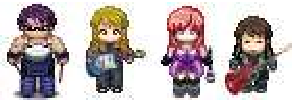
\includegraphics[scale=1]{./Imagenes/grupo.pdf}    
      \end{figure}
  \end{frame}


  \section{Redistribución de las secciones}
    
  \begin{frame}
   \frametitle{Redistribución de secciones}
    \transboxin
 
    \begin{block}{Pautas del profesor}
     El trabajo final que organizará el Revisor lo ordenará de forma que las
     estadísticas sean los primeros trabajos, la evolución de los 
     computadores españoles vengan a continuación y en la última parte 
     estén las características de los demás computadores.
    \end{block}
  
  \begin{block}{Solución}
   La distribución de los temas dada por el coordinador no se vió variada, 
   pero hubo que modificar el orden en que estos temas aparecen.
  
   Esto tampoco influyó en la asignación de trabajos:
   \textsc{tan sólo se vió modificado el número de sección de cada 
   colaborador}.
  
   \begin{itemize}
     \item No se tuvo en cuenta el no modificar el número de sección.
     \item La mayoría de los colaboradores lo corrigieron.
   \end{itemize}
  \end{block}
  
  \end{frame}
 
  
  \section{Revisiones}
  
  \begin{frame}
  \frametitle{Errores comunes}
    \transdissolve
    
  \textsc{No ha habido errores conceptuales}
  
  En general, tan sólo ha habido pequeños errores de estilo o de 
  transcripción:
  
  \begin{itemize}
  \item Confusión de código de secciones.
  \item Faltas ortográficas leves.
  \item Descuadre entre versiones (lógico)
  \end{itemize}
  
  Todos se corrigieron en la revisión final (espero)
  
  \end{frame}
  
  \section{Agradecimientos}
  
  \begin{frame}
  \frametitle{Agradecimientos}
    \transdissolve
    
  \begin{itemize}
  \item Prontitud
  \item Interés
  \item Colaboración
  \end{itemize}
  
  \vspace*{1cm}
  
  A todos los colaboradores: enhorabuena por el trabajo realizado

  \end{frame}
  
 \end{document}
